\section{Classificação de recursos no \emph{middleware uOS}}
\label{sec:classificacaoNoUos}

O \emph{uOS} é um \emph{middleware} cujo propósito é fornecer uma infra-estrutura de \emph{software} utilizando conceitos de computação ubíqua com foco na adaptabilidade de serviços. Seguindo a arquitetura \emph{DSOA}, o \emph{uOS} é responsável por dar suporte ao desenvolvimento de \emph{drivers} e aplicações. Além disso, o \emph{uOS} utiliza o conjunto de protocolos \emph{uP} para realizar sua comunicação.

\begin{figure}[ht]
	\center
	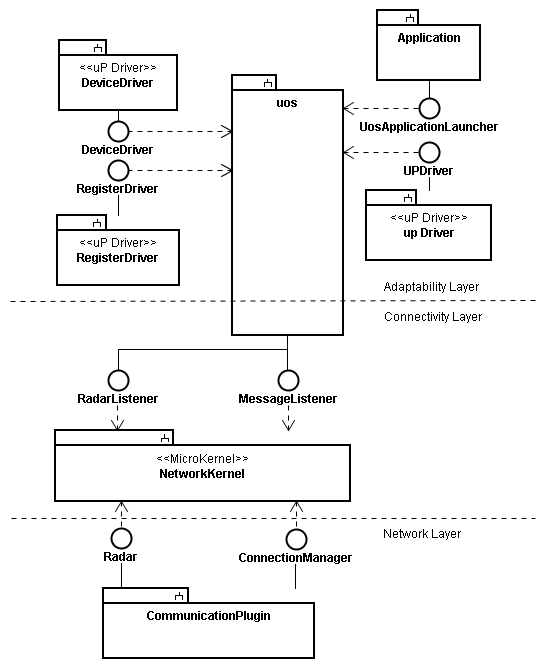
\includegraphics[scale=0.6]{imagens/arquiteturaDoMiddlewareUOS}
	\caption{Diagrama de interação entre as camadas.}
	\label{fig:camadasUOS}
\end{figure}

No sistema destacam-se três camadas: Rede, Conectividade e Adaptabilidade como mostra a Figura~\ref{fig:camadasUOS}. A camada de adaptabilidade é responsável pela coordenação de interações feitas por meio do \emph{middleware}. A Figura~\ref{fig:diagramaDeBlocos} mostra a arquitetura interna da camada de adaptabilidade do \emph{uOS}. A ela adicionou-se uma estrutura em forma de floresta, em que a raiz de cada árvore representa um recurso novo que não é equivalente a nenhum outro. Essa estrutura é inicializada com cada tipo básico (conforme definido na Seção~\ref{sec:tiposBasicos}) compondo uma nova raiz da estrutura de árvores. Este componente é responsável por manter as relações de equivalência dos recursos, mantendo a consistência de serviços e interfaces e impedindo que ocorra uma referência circular entre recursos equivalentes. Quando um novo recurso é registrado no \emph{middleware}, são realizadas validações em seu \emph{driver} segundo as relações de equivalência e em seguida o \emph{driver} é adicionado na árvore de equivalência correta.

Além de manter essa estrutura, a camada de adaptabilidade é responsável por popular a ontologia do \emph{uOS}. O novo \emph{driver} é adicionado à ontologia utilizando um conjunto de interfaces que permite a manipulação estrutural e semântica da ontologia de contexto do \emph{uOS}~\cite{ozakisbcup2011}. Na Figura~\ref{fig:ontologiaUOS} observa-se uma ontologia que contém as classes dos recursos \emph{Pointer} e \emph{Keyboard}.

\begin{figure}[ht]
	\center
	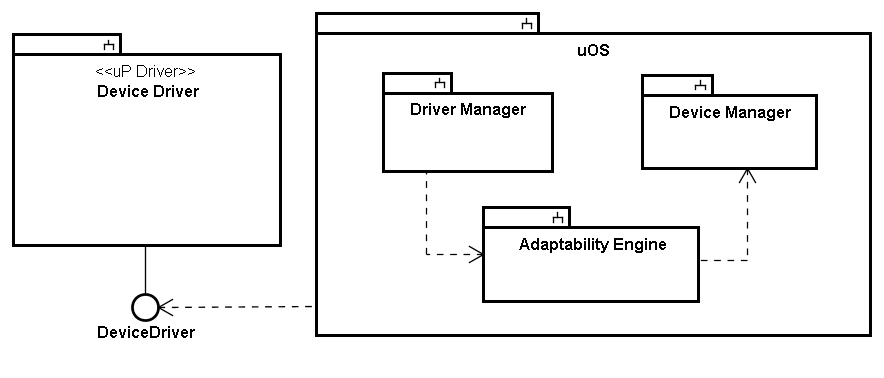
\includegraphics[scale=0.6]{imagens/diagramaDeBlocos}
	\caption{Arquitetura interna da camada de adaptabilidade do \emph{uOS}.}
	\label{fig:diagramaDeBlocos}
\end{figure}

\begin{figure}[ht]
	\center
	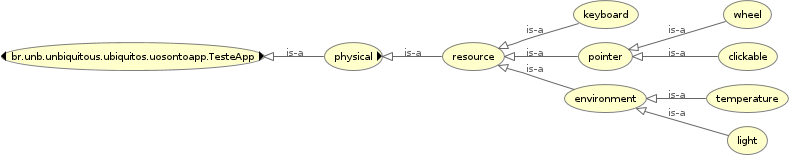
\includegraphics[scale=0.7]{imagens/ontologia}
	\caption{Exemplo de recursos da Ontologia do \emph{uOS}.}
	\label{fig:ontologiaUOS}
\end{figure}

O processo de \emph{handshake}, no qual ocorre a descoberta de novos recursos do ambiente, foi alterado visando tratar os casos em que equivalências desconhecidas são encontradas. Visando um melhor desempenho, foi adicionada uma nova fase ao processo para se tratar estes casos. Quando um novo \emph{driver} a ser registrado é equivalente a pelo menos um desconhecido, ele não será registrado em sua árvore de equivalência enquanto o \emph{driver} desconhecido não for apresentado, ou seja, enquanto as interfaces dos seus recursos não se tornarem conhecidas. Desta forma, cada recurso desconhecido deve ser registrado para somente então registrar o novo recurso na árvore de equivalência.
